%%=============================================================================
%% Methodologie
%%=============================================================================

\chapter{Methodologie}
\label{ch:methodologie}

%% TODO: Hoe ben je te werk gegaan? Verdeel je onderzoek in grote fasen, en
%% licht in elke fase toe welke stappen je gevolgd hebt. Verantwoord waarom je
%% op deze manier te werk gegaan bent. Je moet kunnen aantonen dat je de best
%% mogelijke manier toegepast hebt om een antwoord te vinden op de
%% onderzoeksvraag.

\section{Requirements-analyse}
Om een goede analyse te maken van beide frameworks moeten er requirements opgesteld worden. Aan de hand van deze requirements zullen de frameworks beoordeeld worden. De requirements bestaan uit functionele en niet-functionele requirements. Beide frameworks zullen een score toegewezen krijgen voor elk van de requirements. De scores gaan van 1(zwak) tot 5(uitstekend).

\begin{itemize}
\item  Functionele requirements 
\begin{itemize}
	\item Ondersteuning voor mobile
	\item Compatibiliteit met verschillende browsers
	\item Uitgebreide mogelijkheden rond testing
	\item Beschikbare voorgedefiniëerde componenten 
	\item Ondersteuning voor data binding
	\item Goede performantie
\end{itemize}

\item Niet-functionele requirements
\begin{itemize}
	\item Moet over een goede documentatie beschikken
	\item Moet over een grote community beschikken
	\item Moet relatief makkelijk aan te leren zijn 
	\item Moet open source zijn	
\end{itemize}
\end{itemize}

Deze functionele en niet-functionele requirements zullen nu ingedeeld worden volgens de MoSCoW methode.\autocite{ProductPlan2019}
De 'Must-have initiatives' zijn noodzakelijk voor het framework en moeten dus aanwezig zijn.
De 'Should-have initiatives' zijn een stapje lager dan de must-haves. Ze zijn belangrijk voor het framework maar niet noodzakelijk.
Ten slotte zijn er nog de 'Could-have initiatives'. Deze mogen omschreven worden als nice-to-have. Het is positief indien een framework hieraan voldoet, maar het is geen noodzakelijkheid.

\begin{itemize}
	\item  Must-have initiatives
	\begin{itemize}
	\item Ondersteuning voor mobile
	\item Compatibiliteit met verschillende browsers
	\item Ondersteuning voor data binding
	\item Moet relatief makkelijk aan te leren zijn
	\item Moet open source zijn	 
	\end{itemize}
	\item Should-have initiatives
	\begin{itemize}
	\item Uitgebreide mogelijkheden rond testing
	\item Beschikbare voorgedefiniëerde componenten 
	\item Goede performantie
	\item Moet over een goede documentatie beschikken
	\end{itemize}
		\item Could-have initiatives
		\begin{itemize}
	\item Moet een populair framework zijn met een grote community
		\end{itemize}
\end{itemize}

Om meer inzicht te krijgen in de materie werd een gelijkaardige contactapplicatie gebouwd in zowel Angular (Zie figuur \ref{fig:ContactapplicatieAngular} ) als Vaadin (Zie figuur \ref{fig:ContactapplicatieVaadin} ). In voorgenoemde applicatie kunnen via een formulier nieuwe contacten toegevoegd worden. Beide applicaties werden verbonden met een Spring Boot backend. Deze programma's zijn beschikbaar op volgende locaties:
\begin{itemize}
	\item Frontend Angular: \url{https://github.com/Beazar/BPAngular}
	\item Spring Boot backend voor Angular: \url{https://github.com/Beazar/BPBackend}
	\item Full stack Vaadin: \url{https://github.com/Beazar/BPVaadin}
\end{itemize}

\begin{figure}[H]
	\centering
	
\includegraphics[width=0.6\linewidth]{AngularApp}
	\caption{Contactapplicatie Angular}
	\label{fig:ContactapplicatieAngular}
\end{figure}

\begin{figure}[H]
	\centering
	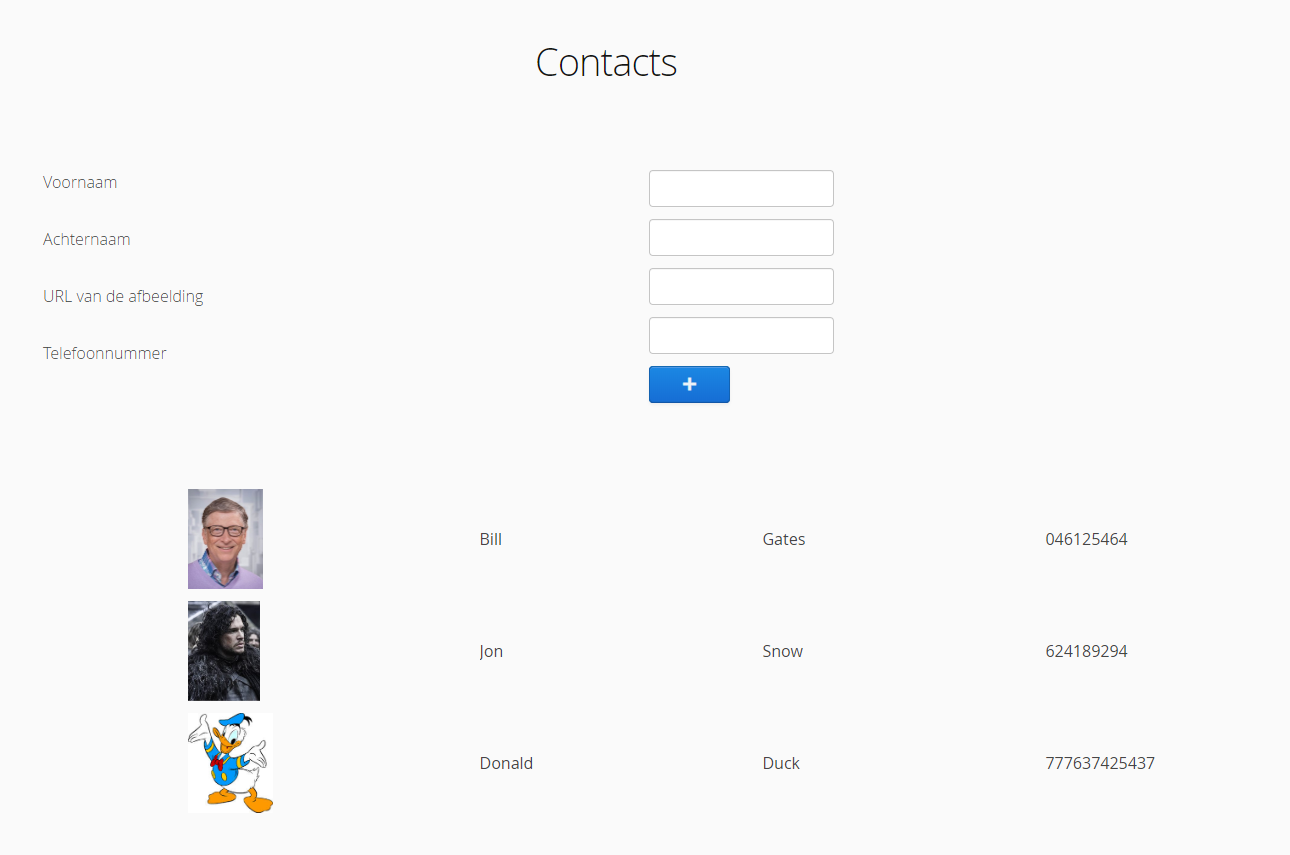
\includegraphics[width=0.6\linewidth]{VaadinApp}
	\caption{Contactapplicatie Vaadin}
	\label{fig:ContactapplicatieVaadin}
\end{figure}

